% CHAPTER 2 OUTLINE
% 2.1 lOGIC eNGINE
%	Intro, give reference to logic engine
%	Explanation of how it works
%	Theorem 2.1.1.
% 2.2 Theorem and Proof to hinged polygons/Squares
% 2.3 Unit Disk Contact Graph



\chapter{Decidability Problems for Hinged Polygons and Unit Disks}
\subsection{The Logic Engine}
\begin{figure}[!htbp]
\begin{center}
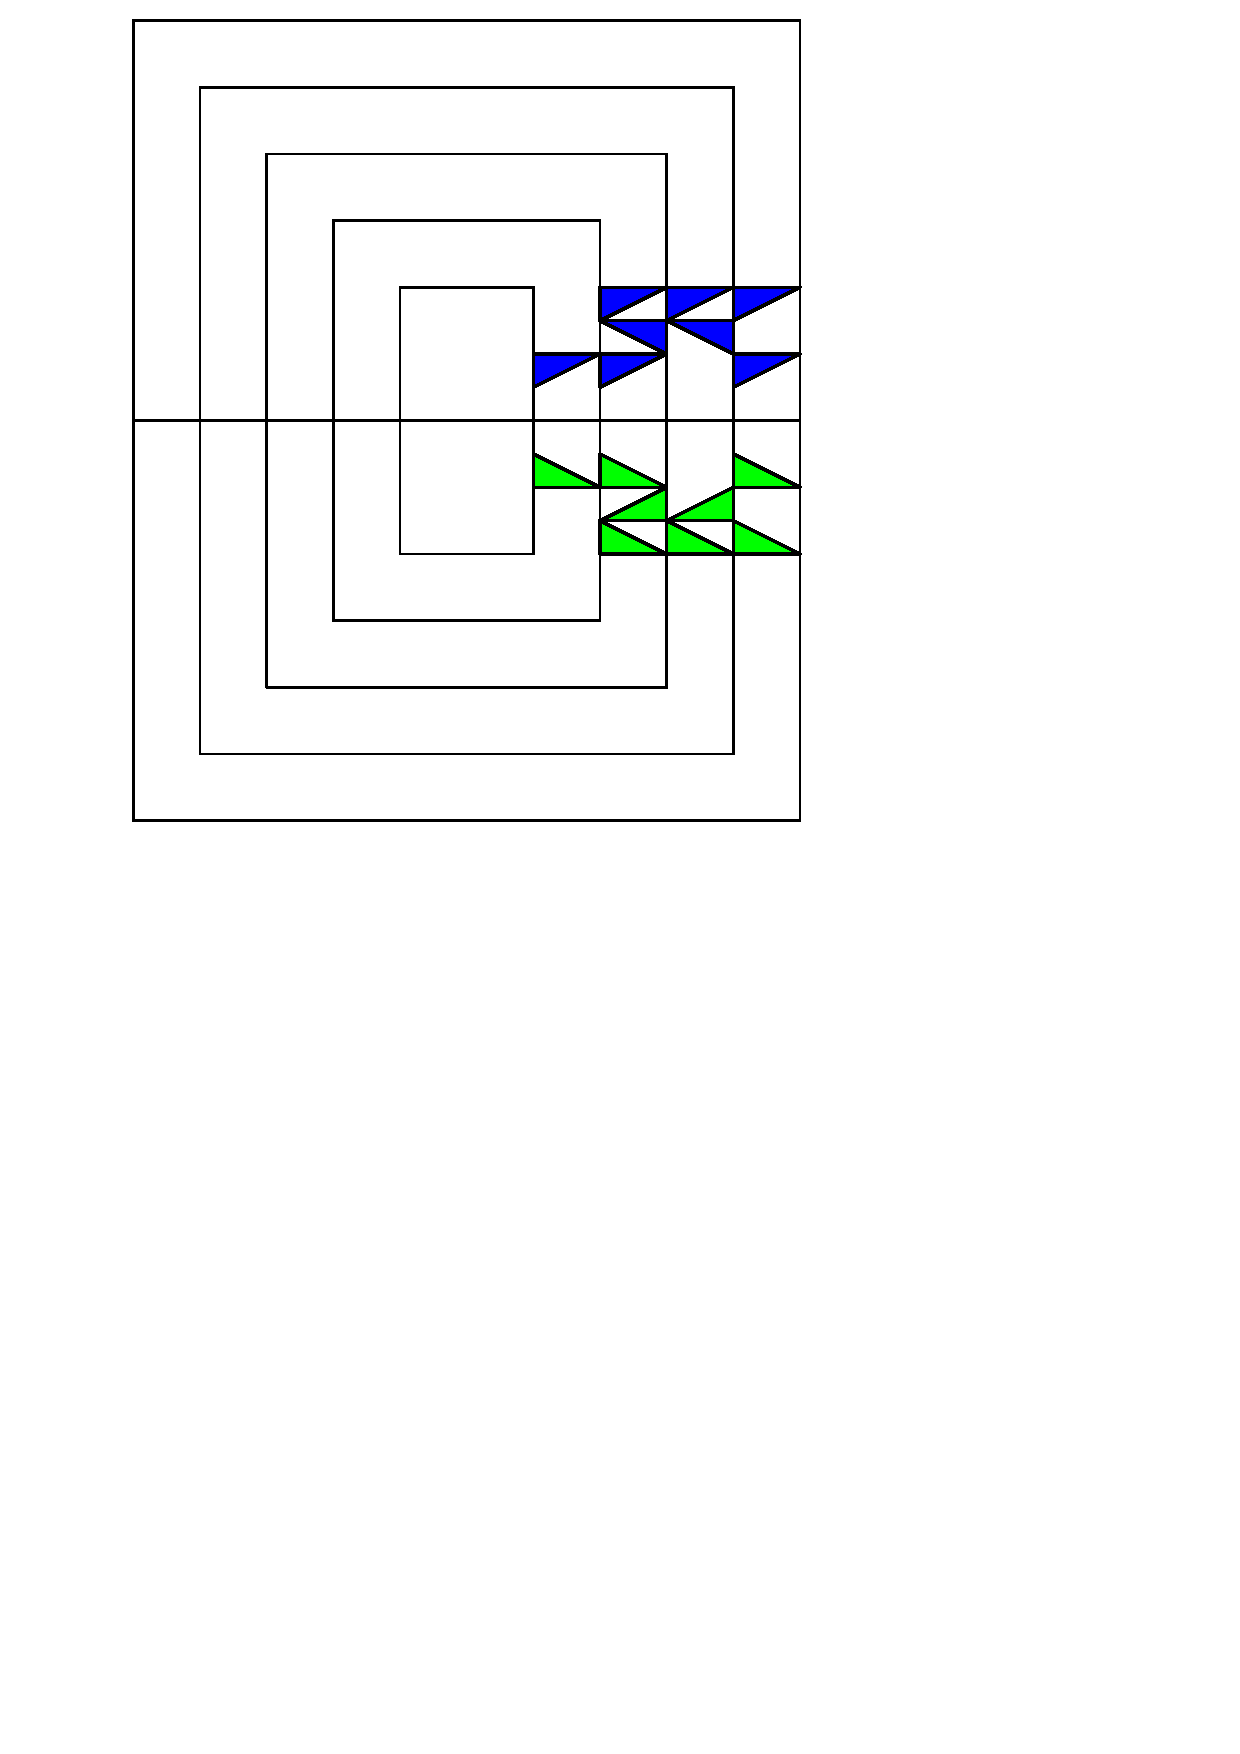
\includegraphics[scale=.66]{graphics/logicengine.pdf}
\caption{A logic engine example.}\label{fig:logicengine-1}
\end{center}
\end{figure}
%add figure of logic engine.
\subsubsection{Construction of the Logic Engine and Encoding of an NAE3SAT Problem on a Logic 
Engine}
% Rigid Frame - A rigid frame that supports the shaft
% Shaft - placed horizontally mid-height of the frame
% Armature - concentric frames contained within the rigid frame supported by the shaft. for each Var
% Chain - for each variable's literal a_j \bar{a}_j,  there exists a chain on that armature
% Flag - flags are for 
The logic engine is a physical model which can encode instances of the NAE3SAT problem.  The 
components of the logic engine are as follows: the rigid frame, the shaft, the armatures,
the chains, and the flags.  Suppose we have an NAE3SAT problem, $P$, with $n$ variables and $m$ 
clauses.  For each variable in $P$, $vj$, there is an \textit{armature}, $A_j$.  The armatures are 
placed concentrically within a \textit{rigid frame}.  A \textit{shaft} placed at mid-height of the 
rigid frame and goes through the armatures.  The armatures can rotate about the shaft.  For each 
clause $C_k$ in $P$, there is are two \textit{links} placed on each armature, $l_{j,k}$ and 
$\bar{l}_{j,k}$. $l_{j,k}$ and $\bar{l}_{j,k}$ place at a height of $k$ and $-k$ respectively on  
each armature.  Every link is flagged except in the case of the following two conditions:
\begin{enumerate}
 \item If the literal $x_j$ is found in clause $C_k$, then $l_{j,k}$ is unflagged.
 \item If the literal $\bar{x}_j$ is found in clause $C_k$, then $\bar{l}_{j,k}$ is unflagged.
\end{enumerate}
A \textit{collision} of flags occur if either of the following occurs:
\begin{enumerate}
\item flags in the same row on adjacent armatures point toward each other.
%display a graphic
\item a flag from the outermost armature $A_n$ points towards the outer rigid frame.
%display a graphic
\item a flag from the innermost armature $A_1$ points inwards of $A_1$.
%display a graphic
\end{enumerate}
\begin{figure}[!htbp]
\begin{center}
\includegraphics[scale=.66]{graphics/logicengineFlags.pdf}
\caption{The blue flags indicate that $x_j$ or $\bar{x}_j$ is not found in clause $C_k$. 
}\label{fig:logicengine-1}
\end{center}
\end{figure}
% 
% 
%   The \textit{rigid frame} is a rectangular enclosure with a horizontal
% shaft place at mid-height.  The \textit{armatures} are concentric rectangular frames contained
% within the rigid frame.  Each armature can rotate about the shaft; other motions on the armature
% are disallowed.  Given an NAE3SAT, for each variable there is a corresponding armature. On each
% armature, there are chains.  A pair of \textit{chains}, $a_j$ and $\bar{a}_j$ correspond to the
% variable $x_j$ and $\bar{x}_j$ respectively.  The pair is placed on each armature, reflected at a
% height of $h$ above and below the shaft, i.e. one place above the shave at a height of $h$, the
% other placed below the shaft at a height of $-h$.
% %insert an armature graphic
% 
% \subsubsection{Encoding the Logic Engine}
% For each clause of an NAE3SAT, there exists a set of corresponding chains, namely the $h^\text{th}$
% clause is the set of chains on the armatures at the $h^\text{th}$ row above and below the shaft. A
% chain is \textit{flagged} if the corresponding variable resides within the clause.  The flag can
% point in either the left or right directions indicating a truth assignment for that variable within
% the clause.  A flag is attached to the $i^\text{th}$ chain of every $a_j^\text{th}$ and
% $\bar{a}_j^\text{th}$ chain with the following exceptions:
% \begin{enumerate}
%  \item if the variable $x_j$  is in clause $C_i$, then link $i$ of $a_j$ is unflagged,
%  \item if the variable $\bar{x}_j$ is in clause $C_i$, then link $i$ of $a_j$ is unflagged.
% \end{enumerate}
\begin{thm}\label{thm:Satisfiability-1}
 An instance of $NAE3SAT$ is a ``yes'' instance if and only if the corresponding logic engine has a
flat, collision-free configuration.
\end{thm}
\begin{pf}
%  If an instance of $NAE3SAT$ is a ``yes'', then every clause in $C$ contains at least one true
% variable and one false variable.  Now suppose the following truth assignment:
Suppose there is an instance of an NAE3SAT problem, $P$, with $n$ variables and $m$ clauses.  Let 
$t$ be a truth assignment to the literals.  If $t \lr{x_1} = 1$, rotate the corresponding armature 
such that $l_{j,k}$ above the shaft and $\bar{l}_{j,k}$ below the shaft.  If $t \lr{x_1} = 0$, 
rotate the corresponding armature such that $l_{j,k}$ is below the shaft and $\bar{l}_{j,k}$ is 
above the shaft.  For each clause $C_k$ there exists a ``true'' and ``false'' literal.  For each 
clause 
there is a correspond pair of rows accross the armatures.  The configuration of those armatures are 
placed such that there is an unflagged link for at least one ``true'' and one ``false'' literal in 
each row.  Configure the flags to point towards the unflagged links. We now have a collision-free 
configuration.

Suppose we have a collision free configuration of a logic engine. We claim that for each row, there 
exists at least one unflagged armature.  To show this, suppose there for any row, there were no 
unflagged armature.  We have two cases:
\begin{enumerate}
 \item Let the flag on $A_1$ point towards $A_n$. Then the flags of $A_2$ through $A_{n-1}$ must 
point towards $A_n$ to be collision free between $A_1$ and $A_{n-1}$.  The flag on $A_n$ cannot 
point toward $A_{n-1}$ otherwise we contradict the hypothesis of the collision free configuration.  
By definition, $A_n$ cannot point towards the outer rigid frame, otherwise results into a 
collision.  

We've shown that there is no collision free row with all armatures flagged in a row.  
To demonstrate that a collision free configuration exists with one flagless armature, suppose $A_i$ 
has a flagless armature.  For all $j$ where $ 1 \leq j < i$, let the flags on $A_j$ point towards 
$A_i$. For all $j$ where $ i < j \leq n$, let the flags on $A_j$ point towards 
$A_i$.  This configuration prevents collision between $A_k$ and $A_{k+1}$ for $k = 1,\dots,n-1$ and 
without loss of generality there is no collision between $A_{i-1}$ and $A_{i+1}$.
\item Let the flag on $A_n$ point towards $A_1$. Then the flags of $A_2$ through $A_{n-1}$ must 
point towards $A_1$ to be collision free between $A_2$ and $A_{n-1}$.  The flag on $A_1$ cannot 
point toward outwards to the rigid frame otherwise we contradict the hypothesis of the collision 
free configuration.  By definition, $A_1$ cannot point inwards, otherwise results into a 
collision.  

We've shown that there is no collision free row with all armatures flagged in a row.  
To demonstrate that a collision free configuration exists with one flagless armature, suppose $A_i$ 
has a flagless armature.  For all $j$ where $ 1 \leq j < i$, let the flags on $A_j$ point towards 
$A_i$. For all $j$ where $ i < j \leq n$, let the flags on $A_j$ point towards 
$A_i$.  This configuration prevents collision between $A_k$ and $A_{k+1}$ for $k = 1,\dots,n-1$ and 
without loss of generality there is no collision between $A_{i-1}$ and $A_{i+1}$.
\end{enumerate}
Since there exists at least one unflagged armature in each row, there 
For flags above the shaft, let each flagged $l_{j,k}$ 
indicate that $x_j$ does not exist in the clause $C_k$.  For flags below the shaft, let each 
flagged link indicate that $\bar{x}_j$ does not exist in the clause.  Let 
$t$ be a truth assignment to the literals.  If $t \lr{x_1} = 1$, rotate the corresponding armature 
such that $l_{j,k}$ above the shaft and $\bar{l}_{j,k}$ below the shaft.  If $t \lr{x_1} = 0$, 
rotate the corresponding armature such that $l_{j,k}$ is below the shaft and $\bar{l}_{j,k}$ is 
above the shaft.  For each clause $C_k$ there exists a ``true'' and ``false'' literal which yields 
a instance of an NAE3SAT is a yes.
\end{pf}

The encoding of the logic engine allows us to make other assertions on other types of 
configurations.
